% !TEX program = lualatex
\documentclass[sn-mathphys-ay]{sn-jnl} % pdflatex/lualatex指定は外してOK

% Prefer bibliography style in the project root (same level as this .tex)
\makeatletter
\def\input@path{{./}}
\makeatother

\usepackage{amsmath,amssymb,amsthm}
\usepackage{graphicx}
\usepackage{booktabs}
\usepackage{xurl} % allow line breaks in long URLs (helps Underfull \hbox in bibliography)
\usepackage{hyperref}
\usepackage{doi}
\Urlmuskip=0mu plus 1mu\relax

% Avoid hyperref PDF-string warnings from TeX-only tokens (e.g., line breaks in titles)
\makeatletter
\pdfstringdefDisableCommands{%
  \def\\{ }%
  \def\comma{, }%
  \def\sep{; }%
  \let\@fnmark\@empty%
}
\makeatother
% Explicit PDF metadata (avoid TeX tokens in PDF strings)
\hypersetup{%
  pdftitle={Decentralized Public R and D, Demand Shifters, and the Over- and Underinvestment Threshold},%
  pdfauthor={Ryota Matsuki}%
}
% Ensure elsarticle's \comma macro is harmless in PDF strings
\makeatletter
\providecommand{\comma}{, }
\makeatother

% --- theorem environments ---
\newtheorem{assumption}{Assumption}
\newtheorem{lemma}{Lemma}
\newtheorem{proposition}{Proposition}
\newtheorem{corollary}{Corollary}
\theoremstyle{remark}
\newtheorem{remark}{Remark}

\raggedbottom
% (optional) suppress underfull box warnings
\hbadness=10000
\vbadness=10000
\begin{document}
% Mitigate small overfull boxes in narrow review layouts
\setlength{\emergencystretch}{2em}

\title[Decentralized Public R\&D, Demand Shifters, and the Over- and Underinvestment Threshold]{Decentralized Public R\&D, Demand Shifters, and the Over- and Underinvestment Threshold}

\author*{\fnm{Ryota} \sur{Matsuki}\thanks{This work was conducted in a personal capacity;\allowbreak\space the views expressed are solely those of the author.}}
\email{ryota.matsuki@gmail.com}

\affil{\orgname{Independent Researcher},
  \orgaddress{\city{Matsuyama}, \state{Ehime}, \country{Japan}}}

\abstract{
We study decentralized public R\&D by local governments when downstream firms compete in prices and policy shifts demand. In a two-jurisdiction Hotelling model, public R\&D raises perceived quality that combines a welfare-relevant (real) component and a purely persuasive component. The welfare-relevant share $\alpha$ determines how much of perceived quality is counted in welfare, while spillovers are governed by $\rho$. Solving downstream Bertrand pricing yields a reduced-form profit function, enabling a closed-form comparison between the decentralized Nash equilibrium and the social optimum. We obtain a sharp sign reversal: decentralized investment is excessive if and only if $\alpha$ is below the cutoff $\bar\alpha(\rho)=2(1-\rho)/[3(1+\rho)]$, and is insufficient above it; in the purely persuasive benchmark ($\alpha=0$), the first best entails zero investment. We also show that the social optimum can be implemented by a single matching instrument on R\&D costs (allowing for negative matching), with an implementing rate $s^*=1-\bar\alpha(\rho)/\alpha$ in closed form. The results clarify when interjurisdictional competition becomes a promotion-policy trap and when knowledge spillovers instead call for coordinated support.




\medskip
\noindent\textit{JEL codes:} H73, H77, L13, O32.
}

\keywords{Decentralized public R\&D\enspace$\cdot$\enspace Matching grants\enspace$\cdot$\enspace Interjurisdictional competition\enspace$\cdot$\enspace Hotelling competition\enspace$\cdot$\enspace Persuasion (advertising)\enspace$\cdot$\enspace Business stealing}

\maketitle

\section{Introduction} 
\label{sec:intro}
Across the world, subnational governments spend public money to “upgrade” and market local products.
Consider a concrete example that is easy to visualize: two neighboring coffee-growing regions that each want to position their beans as \emph{specialty} in export markets.
Both regional governments fund agronomic and processing programs (e.g., disease-resistant varietals, fermentation protocols, quality-control labs, and certification/traceability systems) and also fund branding campaigns (logos, events, slogans, influencer marketing, and tourism tie-ins).%
\footnote{In many agricultural settings, research and promotional activities are administered by \emph{separate} institutions---for example, public experiment stations versus commodity-promotion boards (checkoffs). Our model abstracts from this institutional separation by treating the jurisdiction as a single decision-maker. The two-input extension in Section~\ref{subsec:microfound_alpha} introduces separate decision variables for research and promotion, which partially addresses this concern.}
These interventions raise consumers’ \emph{perceived} quality of a region’s coffee and can be leveraged by downstream firms (e.g., cooperatives and trading firms) competing in prices.
When many jurisdictions pursue similar programs, policy becomes a strategic instrument in \emph{interjurisdictional competition} for demand and local rents.  The resulting externalities---business stealing on one side, knowledge spillovers on the other---share a family resemblance with the fiscal externalities in the tax-competition literature (\citealp{Tiebout1956,Wilson1986,ZodrowMieszkowski1986,Wildasin1988,KeenMarchand1997}), though the mechanism here operates through \emph{product-market demand shifting} rather than competition for mobile capital.%
\footnote{In the standard tax-competition framework, jurisdictions attract mobile capital by lowering tax rates, generating fiscal externalities.  Here, no factor is mobile; instead, public investment shifts demand among differentiated products.  The paper thus sits at the intersection of R\&D competition models (\citealp{dAspremontJacquemin1988,KamienMullerZang1992}) and intergovernmental-grant design (\citealp{Wildasin1984,Wildasin1989}), with public rather than private actors choosing the demand-shifting investment.}
A practical policy question follows: when does decentralized public “R\&D-plus-promotion” create a \emph{promotion-policy trap}---costly spending that mostly reallocates demand across regions---and when does it instead lead to underinvestment because knowledge spillovers are not internalized?\footnote{Many real-world programs bundle welfare-relevant research with generic promotion; for beggar-thy-neighbor incentives in promotion programs, see \citealp{AlstonFreebairnJames2001}.}

A central difficulty is welfare evaluation when policy shifts demand.
Some policy-induced demand shifts reflect real improvements in product quality (better taste, safety, reliability, or verifiable attributes), while others reflect persuasion that changes perceptions without improving underlying quality.
We capture this distinction parsimoniously by decomposing perceived quality into a welfare-relevant (real) component and a purely persuasive component.
A single parameter $\alpha\in[0,1]$ indexes the \emph{welfare-relevant share}: how much of perceived quality is counted in welfare.
This connects our setting to classic welfare analyses of advertising and demand-shifting activities (\citealp{DorfmanSteiner1954,DixitNorman1978}) and to the informative-versus-persuasive distinction in advertising economics (\citealp{Nelson1974,GrossmanShapiro1984,BeckerMurphy1993,Ackerberg2001,BlochManceau1999}).
Intuitively, when $\alpha$ is low (spending is mostly branding/persuasion), interjurisdictional competition tends to look like business stealing; when $\alpha$ is high (spending is mostly quality improvement and verification), the same competition can be socially valuable, especially if knowledge spills over.

We study this trade-off in a two-jurisdiction Hotelling model in which downstream firms compete in prices (Bertrand) and policy affects demand through perceived quality.
Public investment creates a perceived-quality index that spills over across jurisdictions at rate $\rho\in[0,1)$.
Solving the downstream pricing game yields a reduced-form profit function, which allows a closed-form characterization of both the decentralized Nash equilibrium and the social optimum.

Our main results can be stated succinctly:
\begin{itemize}
\item \textbf{Closed-form sign reversal (threshold).}  Decentralized public R\&D is \emph{excessive} if and only if the welfare-relevant share $\alpha$ is below a cutoff that depends on spillovers,
\begin{equation}\label{eq:baralpha}
\bar\alpha(\rho)\equiv \frac{2(1-\rho)}{3(1+\rho)}.
\end{equation}
It is \emph{insufficient} if $\alpha>\bar\alpha(\rho)$. Figure~\ref{fig:regions} summarizes the regions of over- and underinvestment and can be read as a policy-diagnostic chart: the ``overinvestment'' side corresponds to persuasion-heavy (branding/promotion) packages, while the ``underinvestment'' side corresponds to research-heavy (real-quality) packages with spillovers.
\item \textbf{Single-instrument implementation benchmark.} Within the one-dimensional baseline model, a single matching instrument on R\&D costs decentralizes the constrained first best with an implementing rate $s^{*}=1-\bar\alpha(\rho)/\alpha$ in closed form. The required match can be negative, reflecting that when $\alpha$ is sufficiently small, the benchmark calls for restraining (rather than subsidizing) decentralized spending.
\item \textbf{Microfoundation for $\alpha$ (two-input extension).}  We provide a parsimonious extension in which policy has two components: welfare-relevant research and welfare-irrelevant promotion. The extension delivers closed-form allocations and implies that decentralization tilts spending toward persuasion (a \emph{promotion tilt}), thereby lowering the implied welfare-relevant share in closed form. This both clarifies the interpretation of the promotion-policy trap and addresses the concern that $\alpha$ is merely a reduced-form welfare weight.
\end{itemize}

The threshold has a simple economic logic.
A smaller welfare-relevant share magnifies redistributive incentives: when policy mainly persuades rather than improves quality, each jurisdiction has a strong motive to invest in order to steal demand from its rival.
By contrast, stronger spillovers raise the social value of investment relative to private local returns, pushing the distortion toward underinvestment.
In the coffee example, investments in agronomy and verification (quality-control labs, traceability, safety standards) are plausibly high-$\alpha$, whereas spending on slogans, events, and image marketing is plausibly low-$\alpha$.%
\footnote{Geographical indications (GIs) and related certification schemes (PDO/PGI in the EU, GI marks in East Asia) can be interpreted as institutional devices that \emph{raise} the effective $\alpha$ by tying the brand to verifiable production standards. By restricting promotional claims to those backed by certified attributes, GIs also function as \emph{spillover-governance} mechanisms, partly controlling $\rho$ through rules on permitted production area and methods \citep{CrespiMarette2003}. The interplay between GI institutions and the incentives analyzed here is an interesting avenue for future work.}
The model predicts that these two program types can lie on opposite sides of Figure~\ref{fig:regions}: the same interjurisdictional rivalry may be socially productive in one case and socially wasteful in the other.

Finally, although our analysis is theoretical, the key objects admit an empirical interpretation that makes the cutoff operational in principle.
The welfare-relevant share $\alpha$ can be proxied by how much a policy package translates into \emph{objective} quality improvements versus \emph{perception-only} shifts.
High-$\alpha$ components include investments that measurably improve or verify quality (e.g., agronomic and process R\&D, safety and quality-control infrastructure, certification and traceability systems), while low-$\alpha$ components include spending whose primary channel is persuasion (e.g., branding campaigns, slogans, promotional events, influencer marketing).
Empirically, $\alpha$ is thus related to (i) expenditure shares on verifiable quality-improvement/verification versus promotion, and (ii) outcomes such as objective quality scores, certification uptake, safety incidents, and price premia for verified attributes, contrasted with survey-based perception shifts unaccompanied by objective changes.
Spillovers $\rho$ can be proxied by cross-region diffusion of practices and know-how (e.g., adoption patterns, shared extension and training networks, or other diffusion indicators).
These mappings motivate our focus on a closed-form cutoff and a single-instrument rule: the key policy risk is misclassifying the environment (subsidize versus restrain), which is most salient when $\alpha$ is low and spillovers are moderate.

Relative to canonical spillover-driven R\&D models (\citealp{Arrow1962,dAspremontJacquemin1988,Katz1986,KamienMullerZang1992,LeahyNeary1997,Spence1984}) and persuasive-advertising models in differentiated markets (\citealp{BlochManceau1999,Bagwell2007}), the novelty is to combine knowledge spillovers and business-stealing incentives \emph{within a decentralized policy problem} and to close the loop from (i) equilibrium distortion to (ii) implementable intergovernmental matching design (\citealp{Wildasin1984,Wildasin1989}). In addition, Section~\ref{sec:welfare} provides a compact two-input extension that microfounds $\alpha$ by decomposing policy into welfare-relevant research and welfare-irrelevant promotion while preserving the reduced-form profit dependence on the perceived-quality gap.

\begin{figure}[t]
  \centering
  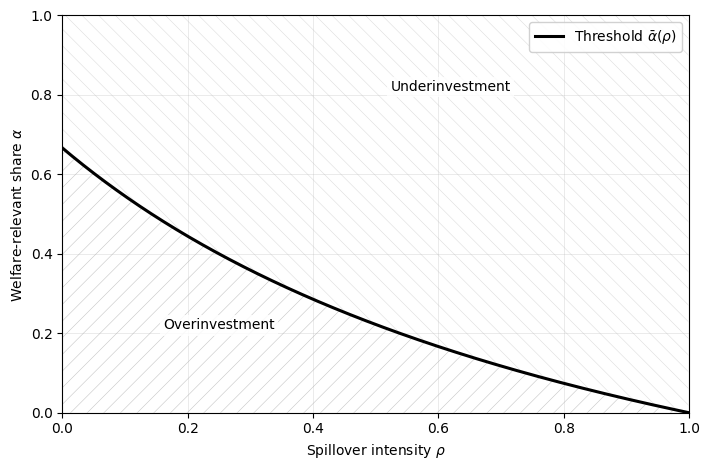
\includegraphics[width=0.8\linewidth]{fig1.png}
  \caption{Regions of over- and underinvestment as a function of spillovers ($\rho$) and the welfare-relevant share ($\alpha$). The solid curve plots the closed-form threshold $\bar\alpha(\rho)=2(1-\rho)/[3(1+\rho)]$ derived in Proposition~\ref{prop:threshold_alpha}.}
  \label{fig:regions}
\end{figure}

The remainder of the paper is organized as follows. Section~\ref{sec:model} presents the model. Section~\ref{sec:price} derives the downstream price equilibrium and the reduced-form profit function. Section~\ref{sec_rd} characterizes the decentralized R\&D equilibrium. Section~\ref{sec:welfare} compares the decentralized outcome to the social optimum, derives the threshold result and implementation, and then presents a two-input extension that microfounds $\alpha$ via real R\&D and promotion. Section~\ref{sec:conclusion} concludes.




\input{model}
\input{price}
\input{sec_rd}
% --- Full English rewrite of the Welfare and Policy section ---

\section{Welfare and Policy}
\label{sec:welfare}

\subsection{Social welfare (fixing the evaluation criterion)}
Social welfare is defined by \eqref{eq:soc_welfare_def}. In accordance with the maintained evaluation criterion, welfare counts only the real component $r_f=\alpha q_f$ and excludes the persuasive component $a_f=(1-\alpha)q_f$ (persuasion does not directly enter welfare).

We interpret $\alpha$ as a reduced-form welfare weight on perceived quality: $\alpha=1$ corresponds to fully welfare-relevant (informative/real) quality, $\alpha=0$ corresponds to purely persuasive demand shifting, and intermediate values allow partial welfare relevance.

\subsection{Preliminaries: market allocation and transport costs (interior region)}
On the interior region, the indifferent location and the resulting market shares satisfy, by Proposition~\ref{prop:price_pers} and Lemma~\ref{lem:xstar},
\begin{equation}\label{eq:xstar_eq}
x^*=\frac{1}{2}+\frac{\Delta q}{6t},
\qquad
D_A^*=x^*,
\qquad
D_B^*=1-x^*,
\qquad (\Delta q\equiv q_A-q_B).
\end{equation}
The transport-cost term is
\begin{equation*}
\int_0^1 t\, d_{\sigma(x)}(x)\,dx
=t\int_0^{x^*} x\,dx+t\int_{x^*}^{1}(1-x)\,dx
=\frac{t}{2}\bigl((x^*)^2+(1-x^*)^2\bigr).
\end{equation*}
Using the identity
\[
(x^*)^2+(1-x^*)^2
=2\left(x^*-\frac{1}{2}\right)^2+\frac{1}{2},
\]
we can rewrite the transport-cost term as
\begin{equation*}
\int_0^1 t\, d_{\sigma(x)}(x)\,dx
=\frac{t}{4}+t\left(x^*-\frac{1}{2}\right)^2.
\end{equation*}
Finally, since \eqref{eq:xstar_eq} implies $x^*-1/2=\Delta q/(6t)$, we obtain
\begin{equation}\label{eq:transport_cost}
\int_0^1 t\, d_{\sigma(x)}(x)\,dx
=\frac{t}{4}+\frac{(\Delta q)^2}{36t}.
\end{equation}

\subsection{The symmetric social optimum (constrained first best)}
\noindent\textit{Terminological note.} Because the planner takes the downstream market structure (Hotelling--Bertrand) and the technology $g$ as given, the resulting optimum is a \emph{constrained first best}: it is first-best conditional on the fixed market structure, not an unconstrained allocation.
\begin{lemma}[Justifying symmetry of the social optimum]\label{lem:soc_symmetry}
Suppose jurisdictions $1$ and $2$ are symmetric and share the same primitives $g$ and $K$. Assume the feasible set $[0,\bar e]^2$ is convex and the planner's objective in \eqref{eq:soc_welfare_def} is concave in $(e_1,e_2)$ on this set (so an optimum exists). Then the planner's problem has at least one symmetric optimal solution with $e_1=e_2$.
\end{lemma}

\begin{proof}
See Appendix~\ref{app:welfare} (Proof of Lemma~\ref{lem:soc_symmetry}).
\end{proof}

\begin{proposition}[FOC for the symmetric social optimum (for the baseline model with $\alpha$)]\label{prop:social_alpha}
By Lemma~\ref{lem:soc_symmetry}, it suffices to focus on symmetric policies $e_1=e_2=e$. If an interior solution exists and $K'$ is increasing while $g'$ is decreasing, then the symmetric social optimum $e^{S}(\alpha)$ is characterized by
\begin{equation}\label{eq:FOC_social_alpha}
K'\!\left(e^{S}(\alpha)\right)=\frac{\alpha(1+\rho)}{2}\,g'\!\left(e^{S}(\alpha)\right).
\end{equation}
In particular, if $\alpha=0$, then $e^{S}(0)=0$.
\end{proposition}
\noindent\textit{Remark.} When $\alpha=0$ (purely persuasive quality), $s^{*}$ in \eqref{eq:sstar} is not defined; implementing $e^{S}(0)=0$ generally requires a sufficiently negative matching rate (i.e., a tax) or an additional instrument, so we restrict attention to $\alpha>0$ in Proposition~\ref{prop:impl}. Note that $s^{*}\to -\infty$ as $\alpha\downarrow 0$, so we restrict attention to $\alpha>0$ in Proposition~\ref{prop:impl}.

\begin{proof}
Under symmetry, $\Delta q=0$ and the allocation is $D_A^*=D_B^*=1/2$. Hence $q_A=q_B=(1+\rho)g(e)$ and welfare-relevant quality equals $\int_0^1 r_{\sigma(x)}dx=\alpha(1+\rho)g(e)$, while transport costs reduce to $t/4$ by \eqref{eq:transport_cost}. Dropping constants, $W^{\mathrm{soc}}(e,e)=\alpha(1+\rho)g(e)-2K(e)+\text{const}$, which yields \eqref{eq:FOC_social_alpha}. A complete derivation is provided in~\ref{app:proof-social}.
\end{proof}

\subsection{A closed-form threshold for over- versus underinvestment}
\begin{proposition}[Real-quality share and the over/underinvestment threshold]\label{prop:threshold_alpha}
Compare the social optimum $e^{S}(\alpha)$ in Proposition~\ref{prop:social_alpha} with the decentralized equilibrium $e^{N}(s)$ in Proposition~\ref{prop:nash_pers}. Let $\bar\alpha$ be defined in \eqref{eq:baralpha}. When $s=0$ (no matching), the following statements hold:
\begin{equation*}
\begin{aligned}
\alpha<\bar\alpha(\rho) \ &\Rightarrow\ e^{N}(0)>e^{S}(\alpha),\\
\alpha=\bar\alpha(\rho) \ &\Rightarrow\ e^{N}(0)=e^{S}(\alpha),\\
\alpha>\bar\alpha(\rho) \ &\Rightarrow\ e^{N}(0)<e^{S}(\alpha).
\end{aligned}
\end{equation*}
Thus, decentralization can entail overinvestment when $\alpha$ is small and underinvestment when $\alpha$ is large.%
\footnote{The specific cutoff $\bar\alpha(\rho)=2(1-\rho)/[3(1+\rho)]$ depends on the Hotelling--Bertrand downstream structure and the linear spillover specification.  Under alternative differentiation models (e.g., Salop circular city, logit demand, or Cournot), the sign-reversal structure---overinvestment for small $\alpha$, underinvestment for large $\alpha$---is expected to survive because it arises from the tension between business-stealing and spillover externalities, which is generic. However, the numerical value of the cutoff and the curvature of the boundary in $(\alpha,\rho)$-space will differ; in this sense, the quantitative predictions are model-specific.}
\end{proposition}

\noindent\textit{Interpretation (business stealing vs.\ spillovers).}
Proposition~\ref{prop:threshold_alpha} isolates a simple tug-of-war between two forces.
On the one hand, when perceived quality is largely \emph{persuasive} (small $\alpha$), local governments spend to steal business from the neighbor, which shows up as a private incentive to raise $e$ even though the welfare-relevant component is small---hence the tendency toward \emph{overinvestment}.
On the other hand, when perceived quality is largely \emph{real} (large $\alpha$), quality improvements generate spillovers across jurisdictions (through $\rho$) that are not fully internalized, so decentralization tends to \emph{underinvest}.
Figure~\ref{fig:regions} below turns this logic into a diagnostic chart.

% (duplicate interpretation block removed)

\medskip
\noindent\textit{Numerical illustration.}
Table~\ref{tab:numerical} evaluates the baseline model under the log-quadratic specification $g(e)=\log(1+e)$, $K(e)=e^2/2$, $t=1$. Several patterns emerge.
When $\alpha$ is small relative to $\bar\alpha(\rho)$ (first two rows), decentralization overinvests---$e^N/e^S>1$---and the corrective matching rate is negative (a tax).
As $\alpha$ rises (rows 3--7), the regime switches to underinvestment and the matching rate becomes a subsidy. Higher spillovers $\rho$ compress the threshold $\bar\alpha(\rho)$ toward zero, making underinvestment the more likely outcome and requiring larger subsidies.


\begin{table}[tbp]
\centering
\caption{Numerical examples: decentralized investment, social optimum, and optimal matching rate.
  Functional forms: $g(e)=\log(1+e)$, $K(e)=e^2/2$, $t=1$.
  The threshold for overinvestment is $\bar\alpha(\rho)=2(1-\rho)/[3(1+\rho)]$.}
\label{tab:numerical}
\smallskip
\begin{tabular}{cccccccc}
\toprule
$\alpha$ & $\rho$ & $\bar\alpha(\rho)$ & $e^N$ & $e^S$ & $e^N/e^S$ & $s^*$ & Regime \\
\midrule
  0.2 & 0.1 & 0.545 & 0.2416 & 0.1000 & 2.42 & -1.727 & over \\
  0.2 & 0.5 & 0.222 & 0.1455 & 0.1325 & 1.10 & -0.111 & over \\
  0.5 & 0.3 & 0.359 & 0.1952 & 0.2583 & 0.76 & +0.282 & under \\
  0.8 & 0.1 & 0.545 & 0.2416 & 0.3307 & 0.73 & +0.318 & under \\
  0.8 & 0.5 & 0.222 & 0.1455 & 0.4220 & 0.34 & +0.722 & under \\
  1.0 & 0.3 & 0.359 & 0.1952 & 0.4487 & 0.44 & +0.641 & under \\
  1.0 & 0.7 & 0.118 & 0.0916 & 0.5488 & 0.17 & +0.882 & under \\
\bottomrule
\end{tabular}
\end{table}


\subsection{Optimal design by the central government (implementation)}
\begin{proposition}[Implementation via matching grants]\label{prop:impl}
Suppose $\alpha>0$. On the relevant interior region, suppose Propositions~\ref{prop:nash_pers} and \ref{prop:social_alpha} apply, and assume that $K'$ is increasing and $g'$ is decreasing. Then the constrained first best $e^{S}(\alpha)$ can be implemented in the decentralized equilibrium by setting the matching rate (possibly negative) $s\in(-\infty,1]$ to
\begin{equation}\label{eq:sstar}
  s^{*}=1-\frac{\bar\alpha(\rho)}{\alpha},
\end{equation}
where $\bar\alpha(\rho)$ is defined in \eqref{eq:baralpha}.%
\footnote{The matching rate $s^{*}$ is financed through lump-sum transfers, so the baseline implementation problem abstracts from any additional deadweight loss of public finance. If, more realistically, public funds carry a shadow cost $\lambda>1$ (reflecting distortionary taxation), the corrective benchmark would generally call for a weaker intervention, because the center would trade off the benefit of correcting the R\&D externality against the cost of raising revenue. We do not solve that richer second-best problem here; the present formula should therefore be read as the clean benchmark under lump-sum finance.}%
\footnote{Throughout, we assume that the central government can \emph{commit} to $s$ before jurisdictions choose $e_i$. If commitment is not feasible---for example, because the center cannot resist ex post renegotiation---the equilibrium matching rate may differ from $s^*$.  In a repeated-game setting, commitment might be sustained by reputation or institutional rules (e.g., multi-year grant programs with preset rates).  The analysis of time-consistent matching policies is left for future work.}
\end{proposition}

\begin{proof}
By Proposition~\ref{prop:nash_pers}, the decentralized equilibrium is characterized by
\begin{equation*}
(1-s)K'\!\left(e^{N}(s)\right)=\frac{1-\rho}{3}\,g'\!\left(e^{N}(s)\right).
\end{equation*}
Dividing both sides by $(1-s)$ gives
\begin{equation*}
K'\!\left(e^{N}(s)\right)=\frac{1-\rho}{3(1-s)}\,g'\!\left(e^{N}(s)\right).
\end{equation*}
By Proposition~\ref{prop:social_alpha}, the social optimum satisfies
\begin{equation*}
K'\!\left(e^{S}(\alpha)\right)=\frac{\alpha(1+\rho)}{2}\,g'\!\left(e^{S}(\alpha)\right).
\end{equation*}
Thus, implementing $e^{N}(s)=e^{S}(\alpha)$ requires
\begin{equation*}
\begin{aligned}
\frac{1-\rho}{3(1-s)}&=\frac{\alpha(1+\rho)}{2}
\iff
1-s=\frac{2(1-\rho)}{3\alpha(1+\rho)}
\iff
s=1-\frac{\bar\alpha(\rho)}{\alpha}.
\end{aligned}
\end{equation*}
which is exactly \eqref{eq:sstar}.
\end{proof}

\noindent\textit{Alternative instruments when $s^{*}$ is strongly negative.}
As $\alpha\downarrow 0$, $s^{*}\to -\infty$: implementing the constrained first best requires arbitrarily large taxes on R\&D---a setting in which the matching-grant mechanism is economically unrealistic. Three complementary policy tools may be considered for this regime:
(i)~\emph{expenditure ceilings}: a direct cap on promotional spending (or equivalently a requirement that a minimum fraction of the budget be allocated to welfare-relevant research);
(ii)~\emph{ex~ante review}: a competitive-grant system in which a central agency evaluates proposed projects and funds only those whose $\alpha$ exceeds a threshold; and
(iii)~\emph{performance-based transfers}: matching payments conditioned on measurable outcomes (e.g., yields, nutritional content) rather than expenditure.
All three approaches restrict or screen the \emph{composition} of investment, complementing---or substituting for---the \emph{level} correction delivered by a matching rate.

\subsection{A two-input extension: microfounding \texorpdfstring{$\alpha$}{alpha} via real R\&D and promotion}
\label{subsec:microfound_alpha}

The baseline model and the present extension play different but complementary roles.
In Sections 2--5.5, the policy problem is one-dimensional and $\alpha$ is treated as an exogenous reduced-form summary of how much of the demand shifter is welfare-relevant; within that benchmark, the single matching rule $s^*=1-\bar\alpha(\rho)/\alpha$ provides a closed-form implementation result.
Section 5.6 moves to a richer environment in which the composition of policy is itself endogenous, so that $\alpha$ is no longer primitive; in that setting, the baseline formula should be read as a benchmark for the one-instrument problem, whereas full efficiency generally requires separate instruments for research and promotion.

We keep the same downstream environment and the reduced-form profit dependence on the perceived-quality gap $\Delta q$ (Corollary~\ref{cor:profit_pers}). We now decompose perceived quality into a welfare-relevant research component and a welfare-irrelevant promotional component:
\[
q_i = q_i^R + q_i^M,\qquad
q_i^R = r_i + \rho_R r_j,\qquad
q_i^M = m_i + \rho_M m_j,\qquad i\neq j,
\]
where $\rho_R,\rho_M\in[0,1)$ capture spillovers in each component. Local governments choose $(r_i,m_i)$ and incur quadratic costs. The decentralized objective is
\[
W_i^G=\pi_i^*(\Delta q)-\frac{k_R}{2}r_i^2-\frac{k_M}{2}m_i^2,
\]
where $\pi_i^*(\Delta q)$ is the same reduced-form profit as in \eqref{eq:profit_red}. Social welfare follows the maintained criterion: only the real component enters welfare directly (promotion is pure persuasion), while market allocation depends on $q_i=q_i^R+q_i^M$ through $\Delta q$.

\begin{proposition}[Two-input allocations under decentralization and under the planner]
\label{prop:two_input}
Consider the interior region $|\Delta q|<3t$ and suppose each government's objective is strictly concave in $(r_i,m_i)$ (Appendix~D provides a sufficient condition). Then the symmetric decentralized equilibrium satisfies
\[
r^N=\frac{1-\rho_R}{3k_R},\qquad
m^N=\frac{1-\rho_M}{3k_M}.
\]
The symmetric social optimum satisfies
\[
r^S=\frac{1+\rho_R}{2k_R},\qquad
m^S=0.
\]
Hence decentralization underprovides welfare-relevant research ($r^N<r^S$) and overprovides purely persuasive promotion ($m^N>m^S$).
\end{proposition}

\begin{corollary}[Endogenous welfare-relevant share (promotion tilt)]
\label{cor:alpha_endog}
In the symmetric decentralized equilibrium, the implied welfare-relevant share of perceived quality is
\[
\alpha^N \equiv \frac{q^R}{q^R+q^M}
=
\frac{k_M(1-\rho_R^2)}{k_M(1-\rho_R^2)+k_R(1-\rho_M^2)}.
\]
In particular, a higher spillover in real research ($\rho_R$) reduces $\alpha^N$ (a stronger tilt toward persuasion), strengthening the promotion-policy trap interpretation of the baseline threshold analysis.
\end{corollary}

\begin{corollary}[Comparative statics of the endogenous welfare-relevant share]\label{cor:alpha_compstatics}
Under the same conditions as Corollary~\ref{cor:alpha_endog}:
\[
\frac{\partial \alpha^N}{\partial k_R}<0,\qquad
\frac{\partial \alpha^N}{\partial k_M}>0,\qquad
\frac{\partial \alpha^N}{\partial \rho_R}<0,\qquad
\frac{\partial \alpha^N}{\partial \rho_M}>0.
\]
Costlier research or larger research spillovers tilt the policy mix toward promotion (lower $\alpha^N$), while costlier promotion or larger promotion spillovers tilt it toward research (higher $\alpha^N$).
\end{corollary}

\begin{proof}
Direct differentiation of $\alpha^N$ in Corollary~\ref{cor:alpha_endog}. In particular,
\[
\frac{\partial\alpha^N}{\partial\rho_R}
=-\frac{2\rho_R\, k_M\, k_R\,(1-\rho_M^2)}{[k_M(1-\rho_R^2)+k_R(1-\rho_M^2)]^2}<0,
\qquad
\frac{\partial\alpha^N}{\partial\rho_M}
=\frac{2\rho_M\, k_M\, k_R\,(1-\rho_R^2)}{[k_M(1-\rho_R^2)+k_R(1-\rho_M^2)]^2}>0.
\]
The signs for $k_R$ and $k_M$ are analogous.
\end{proof}

\noindent\textit{Economic interpretation.}
The result $\partial\alpha^N/\partial k_M>0$ suggests that any development---such as the growth of social media---that \emph{lowers} the unit cost of promotional activity ($k_M\downarrow$) will deepen the promotion tilt and lower $\alpha^N$, thereby pushing the economy further into the overinvestment (promotion-trap) region of Figure~\ref{fig:regions}.

\begin{proposition}[Two-instrument implementation in the two-input model]\label{prop:two_instrument}
Consider the two-input model of Proposition~\ref{prop:two_input}. Suppose a central government can set separate matching rates $s_R$ and $s_M$ on research and promotion costs, so that jurisdiction~$i$ faces effective costs $(1-s_R)\frac{k_R}{2}r_i^2+(1-s_M)\frac{k_M}{2}m_i^2$. Then:
\begin{enumerate}
\item[(i)] The symmetric decentralized equilibrium with matching is
\[
r^N(s_R)=\frac{1-\rho_R}{3k_R(1-s_R)},\qquad
m^N(s_M)=\frac{1-\rho_M}{3k_M(1-s_M)}.
\]
\item[(ii)] The socially optimal research level $r^S=(1+\rho_R)/(2k_R)$ is implemented by setting
\begin{equation}\label{eq:sR_star}
s_R^{*}=1-\frac{2(1-\rho_R)}{3(1+\rho_R)}
=1-\bar\alpha(\rho_R),
\end{equation}
where $\bar\alpha(\cdot)$ is the baseline threshold defined in~\eqref{eq:baralpha}. This has the same structural form as the baseline matching rate $s^{*}$ in~\eqref{eq:sstar} with $\alpha=1$ (because research is 100\% welfare-relevant) and $\rho=\rho_R$.
\item[(iii)] No finite matching rate $s_M$ implements $m^S=0$. Social welfare is strictly decreasing in $s_M$ (since any promotion is pure waste), so the constrained optimum requires either (a)~a direct ban on publicly funded promotion ($m_i=0$), or (b)~a sufficiently negative $s_M$ (a confiscatory tax on promotion costs) to drive $m^N(s_M)$ close to zero.
\end{enumerate}
\end{proposition}

\begin{proof}
Part~(i) follows from the FOC of jurisdiction~1 at symmetry:
\[
\frac{1-\rho_R}{3}=(1-s_R)k_R\, r \quad\Rightarrow\quad r=\frac{1-\rho_R}{3k_R(1-s_R)},
\]
and analogously for $m$.  Part~(ii) equates $r^N(s_R)=r^S$:
\[
\frac{1-\rho_R}{3k_R(1-s_R)}=\frac{1+\rho_R}{2k_R}
\;\Longleftrightarrow\;
1-s_R=\frac{2(1-\rho_R)}{3(1+\rho_R)}=\bar\alpha(\rho_R).
\]
Part~(iii): Since $m^N(s_M)=(1-\rho_M)/[3k_M(1-s_M)]>0$ for all finite $s_M$ (as $\rho_M<1$), no finite rate implements $m^S=0$. Moreover, social welfare is $W^{\mathrm{soc}}=(1+\rho_R)r-k_R r^2-k_M m^2+\mathrm{const}$, and $\partial W/\partial s_M = (\partial W/\partial m)\cdot(\partial m^N/\partial s_M)<0$ because $\partial W/\partial m=-2k_M m<0$ and $\partial m^N/\partial s_M>0$.
\end{proof}

\noindent\textit{Remark.}
The asymmetry between (ii) and (iii) is instructive: matching grants are well suited to correcting the \emph{level} of a welfare-relevant input (research) but cannot eliminate a welfare-irrelevant input (promotion) whose private return is strictly positive. This makes matching grants a necessary but insufficient policy tool in the two-input setting; a quantity regulation or institutional separation (ring-fencing research budgets from promotional budgets) is needed to close the gap.

The extension clarifies the baseline role of $\alpha$: it summarizes the composition of policy between welfare-relevant research and welfare-irrelevant promotion. Even when jurisdictions ``invest a lot'' in the demand shifter $q$, decentralization can be socially wasteful because it reallocates spending toward persuasion and lowers the welfare-relevant share.


\input{conclusion}
\appendix

\section{Proofs for Section~\ref{sec:price}}
\label{app:price}

\begin{proof}[Proof of Lemma~\ref{lem:interior_local}]
\label{app:proof-interior}
(1) If $e_1=e_2=\tilde e$, then \eqref{eq:qi} implies $q_A=g(\tilde e)+\rho g(\tilde e)=q_B$, hence $\Delta q=0$. Substituting $\Delta q=0$ into Proposition~\ref{prop:price_pers} yields $p_A^*=p_B^*=c+t$ and $D_A^*=D_B^*=1/2$, which is interior.

(2) The mapping $\Delta q(e_1,e_2)=(1-\rho)\{g(e_1)-g(e_2)\}$ is continuous because $g$ is continuous, and it satisfies $\Delta q(\tilde e,\tilde e)=0$. By the definition of continuity, there exists $\varepsilon>0$ such that $\|(e_1,e_2)-(\tilde e,\tilde e)\|<\varepsilon$ implies $|\Delta q(e_1,e_2)|<3t$. This inequality guarantees interior demand (equivalently $D_A^*\in(0,1)$), so Proposition~\ref{prop:price_pers} and Corollary~\ref{cor:profit_pers} apply in this neighborhood.

(3) The bound follows immediately from $\Delta q=(1-\rho)\{g(e_1)-g(e_2)\}$ and $e_i\in[0,\bar e]$. If \eqref{eq:global_interior_suff} holds, then $|\Delta q|<3t$ for every feasible profile, which in turn justifies uniqueness of the interior equilibrium and the global use of the reduced-form profits and chain-rule differentiation.
\end{proof}

\begin{proof}[Proof of Corollary~\ref{cor:profit_pers}]
\label{app:proof-profit-red}
Let $\Delta q\equiv q_A-q_B$. By Proposition~\ref{prop:price_pers},
\[
p_A^*-c=t+\frac{\Delta q}{3},
\qquad
D_A^*=\frac{1}{2}+\frac{\Delta q}{6t}.
\]
Therefore,
\[
\pi_A^*=(p_A^*-c)D_A^*
=\left(t+\frac{\Delta q}{3}\right)\left(\frac{1}{2}+\frac{\Delta q}{6t}\right)
=\frac{t}{2}+\frac{\Delta q}{3}+\frac{\Delta q^2}{18t}.
\]
On the other hand,
\[
\frac{(3t+\Delta q)^2}{18t}
=\frac{9t^2+6t\Delta q+\Delta q^2}{18t}
=\frac{t}{2}+\frac{\Delta q}{3}+\frac{\Delta q^2}{18t}.
\]
Hence $\pi_A^*=(3t+\Delta q)^2/(18t)$. The expression for $\pi_B^*$ follows analogously.
\end{proof}


\begin{proof}[Proof of Proposition~\ref{prop:price_pers}]
\label{app:proof-price-pers}
By Lemma~\ref{lem:xstar}, on the interior region demands are $D_A=x^*$ and $D_B=1-x^*$. Hence profits are
\[
\begin{aligned}
\pi_A&=(p_A-c)\frac{q_A-q_B-p_A+p_B+t}{2t},\\
\pi_B&=(p_B-c)\frac{-q_A+q_B+p_A-p_B+t}{2t}.
\end{aligned}
\]
Consider firm $A$. Since $\partial D_A/\partial p_A=-1/(2t)$, its first-order condition is
\[
\frac{\partial \pi_A}{\partial p_A}
= D_A + (p_A-c)\frac{\partial D_A}{\partial p_A}
=\frac{q_A-q_B+c-2p_A+p_B+t}{2t}.
\]
Analogously,
\[
\frac{\partial \pi_B}{\partial p_B}
=\frac{-q_A+q_B+c+p_A-2p_B+t}{2t}.
\]
The second-order conditions hold because
\[
\frac{\partial^2 \pi_A}{\partial p_A^2}=-\frac{1}{t}<0,\qquad
\frac{\partial^2 \pi_B}{\partial p_B^2}=-\frac{1}{t}<0.
\]
Solving the first-order conditions,
\[
q_A-q_B+c-2p_A+p_B+t=0,\qquad
-q_A+q_B+c+p_A-2p_B+t=0,
\]
yields the unique Nash equilibrium,
\[
p_A^*=c+t+\frac{q_A-q_B}{3},\qquad
p_B^*=c+t-\frac{q_A-q_B}{3}.
\]
Substituting into \eqref{eq:xstar_general} delivers \eqref{eq:shares}.
\end{proof}




\section{Proofs for Section~\ref{sec_rd}}
\label{app:rd}


% Ensure starred subsections can be referenced without producing "B.1"-style numbering
\renewcommand{\thesubsection}{\Alph{section}}

% Ensure starred subsections can be referenced without producing "B.1"-style numbering
\renewcommand{\thesubsection}{\Alph{section}}






\subsection*{A sufficient condition for strict concavity}
\label{app:concavity}
On the interior region, $\pi_i^*$ is a quadratic function of $\Delta q$ as in \eqref{eq:profit_red}, with $\Delta q=(1-\rho)\{g(e_i)-g(e_j)\}$ by \eqref{eq:Delta_q}. Holding $e_j$ fixed and differentiating yields

\[
\frac{\partial^2 \pi_i^*}{\partial e_i^2}
=\frac{1}{9t}\Bigl((1-\rho)^2\{g'(e_i)\}^2+(1-\rho)\{3t\pm \Delta q\}g''(e_i)\Bigr)
\le \frac{(1-\rho)^2}{9t}\{g'(e_i)\}^2,
\]
where the inequality uses $g''\le 0$. Thus, under $s<1$, if
\[
(1-s)K''(e_i)>\frac{(1-\rho)^2}{9t}\{g'(e_i)\}^2 \quad \text{for all }e_i\in[0,\bar e],
\]
then $W_i^{\mathrm{loc}}=\pi_i^*-(1-s)K$ is strictly concave in $e_i$. For instance, if $g(e)=\beta\log(1+e)$ and $K(e)=\frac{\kappa}{2}e^2$, then $g'(e)\le \beta$ implies that $(1-s)\kappa>\frac{(1-\rho)^2}{9t}\beta^2$ is sufficient.

\begin{proof}[Proof of Proposition~\ref{prop:nash_pers}]
\label{app:proof-nash}
By Lemma~\ref{lem:interior_local}, on the interior region the reduced-form profits in Corollary~\ref{cor:profit_pers} apply, and differentiation via the chain rule is valid. Jurisdiction $1$ maximizes
\[
W_1^{\mathrm{loc}}(e_1,e_2)=\pi_A^*(q_A,q_B)-(1-s)K(e_1).
\]
Differentiating with respect to $e_1$ gives
\begin{equation}\label{eq:dWdx_general}
\frac{\partial W_1^{\mathrm{loc}}}{\partial e_1}
=\frac{\partial \pi_A^*}{\partial \Delta q}\cdot\frac{\partial \Delta q}{\partial e_1}-(1-s)K'(e_1).
\end{equation}
From Corollary~\ref{cor:profit_pers},
\[
\pi_A^*=\frac{(3t+\Delta q)^2}{18t}
\quad\Rightarrow\quad
\frac{\partial \pi_A^*}{\partial \Delta q}=\frac{3t+\Delta q}{9t}.
\]
Moreover, \eqref{eq:Delta_q} implies
\[
\frac{\partial \Delta q}{\partial e_1}=(1-\rho)g'(e_1).
\]
Substituting into \eqref{eq:dWdx_general} yields
\[
\frac{\partial W_1^{\mathrm{loc}}}{\partial e_1}
=\frac{3t+\Delta q}{9t}(1-\rho)g'(e_1)-(1-s)K'(e_1).
\]
At a symmetric profile $e_1=e_2=e$, we have $\Delta q=0$, so
\[
\left.\frac{\partial W_1^{\mathrm{loc}}}{\partial e_1}\right|_{e_1=e_2=e}
=\frac{3t}{9t}(1-\rho)g'(e)-(1-s)K'(e)
=\frac{1-\rho}{3}g'(e)-(1-s)K'(e).
\]
Imposing the first-order condition $\partial W_1^{\mathrm{loc}}/\partial e_1=0$ gives \eqref{eq:FOC_nash_pers}. If $K'(0)=0$ and $g'(0)>0$, then the right-hand side of \eqref{eq:FOC_nash_pers} is strictly positive at $e=0$ whereas the left-hand side equals zero; monotonicity therefore implies $e^{N}(s)>0$. Uniqueness follows from Assumption~\ref{ass:concave_pers} together with standard monotonicity arguments.
\end{proof}

\section{Proofs for Section~\ref{sec:welfare}}
\label{app:welfare}

\begin{proof}[Proof of Lemma~\ref{lem:soc_symmetry}]
\label{app:proof-soc-sym}
The welfare function \eqref{eq:soc_welfare_def} is invariant to relabeling ($1\leftrightarrow 2$). Hence, if $(e_1,e_2)$ is optimal, then so is the swapped profile $(e_2,e_1)$, yielding the same welfare level. If the feasible set is convex and the objective is concave in $(e_1,e_2)$ (a convenient sufficient condition), then the average profile $(\frac{e_1+e_2}{2},\frac{e_1+e_2}{2})$ achieves at least the same welfare. Therefore, a symmetric optimum exists.
\end{proof}


\begin{proof}[Proof of Proposition~\ref{prop:social_alpha}]
\label{app:proof-social}
Under a symmetric policy $e_1=e_2=e$, \eqref{eq:qi} implies
\[
q_A=q_B=(1+\rho)g(e),
\qquad
\Delta q=0,
\qquad
D_A^*=D_B^*=\frac12.
\]
Moreover, by \eqref{eq:decompose}, $r_A=r_B=\alpha(1+\rho)g(e)$, so
\[
\int_0^1 r_{\sigma(x)}\,dx
=r_A D_A^*+r_B D_B^*
=\alpha(1+\rho)g(e)\cdot \frac12+\alpha(1+\rho)g(e)\cdot \frac12
=\alpha(1+\rho)g(e).
\]
Transport costs equal $t/4$ by substituting $\Delta q=0$ into \eqref{eq:transport_cost}. Dropping constants, we can write
\[
W^{\mathrm{soc}}(e,e)=\alpha(1+\rho)g(e)-2K(e)-\frac{t}{4}+\text{const}.
\]
The first-order condition is therefore
\[
\frac{d}{de}W^{\mathrm{soc}}(e,e)=\alpha(1+\rho)g'(e)-2K'(e)=0,
\]
which is equivalent to \eqref{eq:FOC_social_alpha}. When $\alpha=0$, the condition reduces to $-2K'(e)=0$, and since $K'(e)>0$ for $e>0$, it follows that $e^{S}(0)=0$.
\end{proof}
\section*{Appendix D Proofs for Section~\ref{subsec:microfound_alpha} (two-input extension)}

\subsection*{D.1 Reduced-form profit derivative}
From Corollary~\ref{cor:profit_pers}, for seller $A$ the reduced-form equilibrium profit on the interior region is $\pi_A^*(\Delta q)=(3t+\Delta q)^2/(18t)$, hence
\[
\frac{\partial \pi_A^*}{\partial \Delta q}=\frac{3t+\Delta q}{9t},\qquad
\left.\frac{\partial \pi_A^*}{\partial \Delta q}\right|_{\Delta q=0}=\frac13.
\]

\subsection*{D.2 Perceived-quality gap in $(r,m)$}
By construction,
\[
\Delta q = (q_i^R+q_i^M)-(q_j^R+q_j^M)
=(1-\rho_R)(r_i-r_j)+(1-\rho_M)(m_i-m_j),
\]
so $\partial \Delta q/\partial r_i=1-\rho_R$ and $\partial \Delta q/\partial m_i=1-\rho_M$.

\subsection*{D.3 Decentralized FOCs and symmetric equilibrium}
Government $i$ maximizes
\[
W_i^G=\pi_i^*(\Delta q)-\frac{k_R}{2}r_i^2-\frac{k_M}{2}m_i^2.
\]
Using the chain rule, evaluated at the symmetric point $\Delta q=0$,
\[
0=\frac{\partial W_i^G}{\partial r_i}
=\left.\frac{\partial \pi_i^*}{\partial \Delta q}\right|_{\Delta q=0}(1-\rho_R)-k_R r_i
\ \Rightarrow\ r^N=\frac{1-\rho_R}{3k_R},
\]
and analogously $m^N=(1-\rho_M)/(3k_M)$.

\subsection*{D.4 Concavity condition (sufficient)}
Since $\pi_i^*(\Delta q)$ is convex in $\Delta q$ with $\partial^2 \pi_i^*/\partial \Delta q^2=1/(9t)$ and $\Delta q$ is linear in $(r_i,m_i)$, the Hessian of $W_i^G$ with respect to $(r_i,m_i)$ is
\[
H_i=\frac{1}{9t}
\begin{pmatrix}
(1-\rho_R)^2 & (1-\rho_R)(1-\rho_M)\\
(1-\rho_R)(1-\rho_M) & (1-\rho_M)^2
\end{pmatrix}
-
\begin{pmatrix}
k_R & 0\\
0 & k_M
\end{pmatrix}.
\]
A sufficient (and in this rank-one form, also necessary) condition for strict concavity is
\[
\frac{1}{9t}\left(\frac{(1-\rho_R)^2}{k_R}+\frac{(1-\rho_M)^2}{k_M}\right)<1.
\]

\subsection*{D.5 Social optimum and $m^S=0$}
Under the maintained welfare criterion, promotion does not enter welfare directly. At the symmetric point, $\Delta q=0$, so the allocation and transport-cost terms are locally unaffected to first order by a symmetric change in $m$. Therefore,
\[
\left.\frac{\partial W^S}{\partial m_i}\right|_{\text{sym}}=-k_M m_i \ \Rightarrow\ m^S=0.
\]
For research, at symmetry each jurisdiction serves half of consumers and a marginal increase in $r_i$ raises the real component for its own consumers by $1$ and for the other jurisdiction's consumers via the spillover by $\rho_R$. Hence the marginal social gain is $(1+\rho_R)/2$, yielding
\[
\left.\frac{\partial W^S}{\partial r_i}\right|_{\text{sym}}=\frac{1+\rho_R}{2}-k_R r_i \ \Rightarrow\ r^S=\frac{1+\rho_R}{2k_R}.
\]

\subsection*{D.6 Endogenous share}
At symmetry, $q^R=(1+\rho_R)r^N$ and $q^M=(1+\rho_M)m^N$, hence
\[
\alpha^N=\frac{(1+\rho_R)r^N}{(1+\rho_R)r^N+(1+\rho_M)m^N}
=\frac{k_M(1-\rho_R^2)}{k_M(1-\rho_R^2)+k_R(1-\rho_M^2)}.
\]


\section*{Statements and Declarations}

\subsection*{Competing Interests}
The author declares that he has no competing interests.

\subsection*{Funding}
No funding was received to assist with the preparation of this manuscript.

\subsection*{Data availability}
Not applicable. No datasets were generated or analyzed in this study.

\subsection*{Author Contributions}
Ryota Matsuki: conceptualization, formal analysis, writing (original draft), writing (review and editing).

\subsection*{Use of Generative AI and AI-assisted Technologies}
During the preparation of this work, the author used ChatGPT (OpenAI) to (i) brainstorm and refine exposition, (ii) organize related literature, and (iii) obtain suggestions for checking algebraic derivations. The author reviewed and edited the content as needed and takes full responsibility for the manuscript.

% --- Inline bibliography (do NOT require BibTeX processing by submission system) ---
% Generated from bib_complete.bbl (with DOI shown as full https://doi.org/... links)
\begin{thebibliography}{}
\bibitem[Ackerberg(2001)]{Ackerberg2001}
Ackerberg, Daniel A. (2001).
\newblock Empirically Distinguishing Informative and Prestige Effects of Advertising.
\newblock \emph{The RAND Journal of Economics}, 32(2), 316--333.
\newblock \url{https://www.jstor.org/stable/2696412}

\bibitem[Alston et~al.(2001)]{AlstonFreebairnJames2001}
Alston, Julian M., Freebairn, John W., \& James, Jennifer S. (2001).
\newblock Beggar-Thy-Neighbor Advertising: Theory and Application to Generic Commodity Promotion Programs.
\newblock \emph{American Journal of Agricultural Economics}, 83(4), 888--902.
\newblock \url{https://onlinelibrary.wiley.com/doi/abs/10.1111/0002-9092.00217}

\bibitem[Alston et~al.(1995)]{AlstonNortonPardey1995}
Alston, Julian M., Norton, George W., \& Pardey, Philip G. (1995).
\newblock \emph{Science Under Scarcity: Principles and Practice for Agricultural Research Evaluation and Priority Setting}.
\newblock Cornell University Press.
\newblock \url{https://hdl.handle.net/10568/136536}

\bibitem[Alston et~al.(2020)]{AlstonPardeyRao2020}
Alston, Julian M., Pardey, Philip G., \& Rao, Xudong (2020).
\newblock The Payoff to Investing in CGIAR Research.
\newblock University of Minnesota, Department of Applied Economics.
\newblock \url{https://ageconsearch.umn.edu/record/337029}

\bibitem[Arrow(1962)]{Arrow1962}
Arrow, Kenneth J. (1962).
\newblock Economic Welfare and the Allocation of Resources for Invention.
\newblock In Richard R. Nelson (Ed.), \emph{The Rate and Direction of Inventive Activity: Economic and Social Factors} (pp.\ 609--626).
\newblock Princeton University Press.
\newblock \url{https://www.nber.org/books-and-chapters/rate-and-direction-inventive-activity-economic-and-social-factors/economic-welfare-and-allocation-resources-invention}

\bibitem[Bagwell(2007)]{Bagwell2007}
Bagwell, Kyle (2007).
\newblock The Economic Analysis of Advertising.
\newblock In Mark Armstrong \& Robert H. Porter (Eds.), \emph{Handbook of Industrial Organization} (Vol.\ 3, pp.\ 1701--1844).
\newblock Elsevier.
\newblock \url{https://www.sciencedirect.com/science/article/pii/S1573448X06030287}

\bibitem[Becker and Murphy(1993)]{BeckerMurphy1993}
Becker, Gary S. \& Murphy, Kevin M. (1993).
\newblock A Simple Theory of Advertising as a Good or Bad.
\newblock \emph{The Quarterly Journal of Economics}, 108(4), 941--964.
\newblock \url{https://www.jstor.org/stable/2118455}

\bibitem[Bloch and Manceau(1999)]{BlochManceau1999}
Bloch, Francis \& Manceau, Delphine (1999).
\newblock Persuasive Advertising in Hotelling's Model of Product Differentiation.
\newblock \emph{International Journal of Industrial Organization}, 17(4), 557--574.
\newblock \url{https://www.sciencedirect.com/science/article/pii/S0167718798000149}

\bibitem[Crespi and Marette(2003)]{CrespiMarette2003}
Crespi, John M. \& Marette, Stephan (2003).
\newblock Some Economic Implications of Public Labeling.
\newblock \emph{Journal of Food Distribution Research}, 34(3), 1--12.
\newblock \url{https://ageconsearch.umn.edu/record/27053}

\bibitem[d'Aspremont and Jacquemin(1988)]{dAspremontJacquemin1988}
d'Aspremont, Claude \& Jacquemin, Alexis (1988).
\newblock Cooperative and Noncooperative R\&D in Duopoly with Spillovers.
\newblock \emph{American Economic Review}, 78(5), 1133--1137.
\newblock \url{https://www.jstor.org/stable/1807173}

\bibitem[Dixit and Norman(1978)]{DixitNorman1978}
Dixit, Avinash \& Norman, Victor (1978).
\newblock Advertising and Welfare.
\newblock \emph{The Bell Journal of Economics}, 9(1), 1--17.
\newblock \url{https://www.jstor.org/stable/3003609}

\bibitem[Dorfman and Steiner(1954)]{DorfmanSteiner1954}
Dorfman, Robert \& Steiner, Peter O. (1954).
\newblock Optimal Advertising and Optimal Quality.
\newblock \emph{American Economic Review}, 44(5), 826--836.
\newblock \url{https://www.jstor.org/stable/1807704}

\bibitem[Grossman and Shapiro(1984)]{GrossmanShapiro1984}
Grossman, Gene M. \& Shapiro, Carl (1984).
\newblock Informative Advertising with Differentiated Products.
\newblock \emph{Review of Economic Studies}, 51(1), 63--81.
\newblock \url{https://www.jstor.org/stable/2297705}

\bibitem[Hurley et~al.(2014)]{HurleyRaoPardey2014}
Hurley, Terrance M., Rao, Xudong, \& Pardey, Philip G. (2014).
\newblock Re-examining the Reported Rates of Return to Food and Agricultural Research and Development.
\newblock \emph{American Journal of Agricultural Economics}, 96(5), 1492--1504.
\newblock \url{https://academic.oup.com/ajae/article/96/5/1492/2737489}

\bibitem[Kamien et~al.(1992)]{KamienMullerZang1992}
Kamien, Morton I., Muller, Eitan, \& Zang, Israel (1992).
\newblock Research Joint Ventures and R\&D Cartels.
\newblock \emph{American Economic Review}, 82(5), 1293--1306.
\newblock \url{https://www.jstor.org/stable/2117479}

\bibitem[Kinnucan and Zheng(2004)]{KinnucanZheng2004}
Kinnucan, Henry W. \& Zheng, Yuqing (2004).
\newblock Advertising's Effect on the Market Demand Elasticity: A Note.
\newblock \emph{Agribusiness}, 20(2), 181--188.
\newblock \url{https://onlinelibrary.wiley.com/doi/abs/10.1002/agr.20004}

\bibitem[Katz(1986)]{Katz1986}
Katz, Michael L. (1986).
\newblock An Analysis of Cooperative Research and Development.
\newblock \emph{The RAND Journal of Economics}, 17(4), 527--543.
\newblock \url{https://www.jstor.org/stable/2555479}

\bibitem[Keen and Marchand(1997)]{KeenMarchand1997}
Keen, Michael \& Marchand, Maurice (1997).
\newblock Fiscal Competition and the Pattern of Public Spending.
\newblock \emph{Journal of Public Economics}, 66(1), 33--53.
\newblock \url{https://www.sciencedirect.com/science/article/pii/S0047272797000352}

\bibitem[Leahy and Neary(1997)]{LeahyNeary1997}
Leahy, Dermot \& Neary, J. Peter (1997).
\newblock Public Policy towards R\&D in Oligopolistic Industries.
\newblock \emph{American Economic Review}, 87(4), 642--662.
\newblock \url{https://www.jstor.org/stable/2951367}

\bibitem[Nelson(1974)]{Nelson1974}
Nelson, Phillip (1974).
\newblock Advertising as Information.
\newblock \emph{Journal of Political Economy}, 82(4), 729--754.
\newblock \url{https://www.jstor.org/stable/1837143}

\bibitem[Spence(1984)]{Spence1984}
Spence, A. Michael (1984).
\newblock Cost Reduction, Competition, and Industry Performance.
\newblock \emph{Econometrica}, 52(1), 101--121.
\newblock \url{https://www.jstor.org/stable/1911463}

\bibitem[Tiebout(1956)]{Tiebout1956}
Tiebout, Charles M. (1956).
\newblock A Pure Theory of Local Expenditures.
\newblock \emph{Journal of Political Economy}, 64(5), 416--424.
\newblock \url{https://www.jstor.org/stable/1826343}

\bibitem[Wildasin(1984)]{Wildasin1984}
Wildasin, David E. (1984).
\newblock The Welfare Effects of Intergovernmental Grants in an Economy with Distortionary Local Taxes.
\newblock \emph{Journal of Public Economics}, 25(1--2), 103--125.
\newblock \url{https://www.sciencedirect.com/science/article/pii/004727278490046X}

\bibitem[Wildasin(1988)]{Wildasin1988}
Wildasin, David E. (1988).
\newblock Nash Equilibria in Models of Fiscal Competition.
\newblock \emph{Journal of Public Economics}, 35(2), 229--240.
\newblock \url{https://www.sciencedirect.com/science/article/pii/0047272788900552}

\bibitem[Wildasin(1989)]{Wildasin1989}
Wildasin, David E. (1989).
\newblock Interjurisdictional Capital Mobility: Fiscal Externality and a Corrective Subsidy.
\newblock \emph{Journal of Urban Economics}, 25(2), 193--212.
\newblock \url{https://www.sciencedirect.com/science/article/pii/009411908990034X}

\bibitem[Wilson(1986)]{Wilson1986}
Wilson, John Douglas (1986).
\newblock A Theory of Interregional Tax Competition.
\newblock \emph{Journal of Urban Economics}, 19(3), 296--315.
\newblock \url{https://www.sciencedirect.com/science/article/pii/0094119086900458}

\bibitem[Wilson(1999)]{Wilson1999}
Wilson, John Douglas (1999).
\newblock Theories of Tax Competition.
\newblock \emph{National Tax Journal}, 52(2), 269--304.
\newblock \url{https://www.jstor.org/stable/2006731}

\bibitem[Zodrow and Mieszkowski(1986)]{ZodrowMieszkowski1986}
Zodrow, George R. \& Mieszkowski, Peter (1986).
\newblock Pigou, Tiebout, Property Taxation, and the Underprovision of Local Public Goods.
\newblock \emph{Journal of Urban Economics}, 19(3), 356--370.
\newblock \url{https://www.sciencedirect.com/science/article/pii/0094119086900483}

\end{thebibliography}
\end{document}
